% Copyright (C) 2005-2015 Airbus - EDF - IMACS - Phimeca
% Permission is granted to copy, distribute and/or modify this document
% under the terms of the GNU Free Documentation License, Version 1.2
% or any later version published by the Free Software Foundation;
% with no Invariant Sections, no Front-Cover Texts, and no Back-Cover
% Texts.  A copy of the license is included in the section entitled "GNU
% Free Documentation License".
\renewcommand{\filename}{docUC_InputWithData_EmpiricalDrawing.tex}
\renewcommand{\filetitle}{UC : Drawing Empirical CDF, Histogram, Clouds / PDF or superposition of two clouds from data}

% \HeaderNNIILevel
% \HeaderIILevel
\HeaderIIILevel



\index{Graph!Empirical cumulative density function}
\index{Graph!Histogram}
\index{Graph!Superposition two points clouds}
\index{Graph Manipulation!Bounding box}
\index{Graph Manipulation!View}
\index{Graph Manipulation!Show}



The objective of this Use Case is to draw :
\begin{itemize}
\item the empirical cumulative density function (CDF) from data : GRAPH 1,
\item the histogram from data : GRAPH 2 (with imposed number of bars) and GRAPH 3 (with free number of bars) ,
\item the superposition of two 2D samples where the first sample is given as sample and the second sample is evaluated from a given from a 2D distribution : GRAPH 4,
\item the superposition of two 2D samples where both samples are given as samples : GRAPH 5.
\end{itemize}



Details on empirical cumulative distribution function may be found in the Reference Guide (\extref{ReferenceGuide}{see file Reference Guide - Step B -- Empirical cumulative distribution function}{stepB}).\\



To draw an histogram, it is possible :
\begin{itemize}
\item to fix the number of bars,
\item or not to mention it : OpenTURNS will determine automatically the bandwidth of the histogram according to the Silverman rule (gaussian empirical rule).
\end{itemize}

\requirements{
  \begin{description}
  \item[$\bullet$] one scalar numerical sample : {\itshape sample}
  \item[$\bullet$] two 2D numerical samples : {\itshape sample2, sample3}
  \item[type:] NumericalSample
  \item[$\bullet$] one 2D distribution : {\itshape dist2D}
  \item[type:] Distribution
  \end{description}
}
             {
               \begin{description}
               \item[$\bullet$] the files containing the empirical CDF graph : {\itshape sampleCDF.png, sampleCDF.eps, sampleCDFZoom.png, sampleCDFZoom.eps}
               \item[type:]  files at format PNG or EPS or FIG
               \item[$\bullet$] the files containing the histogram graph : {\itshape sampleHist.png, sampleHist.eps, sampleHistOpt.png, sampleHistOpt.eps}
               \item[type:]  files at format PNG or EPS or FIG
               \item[$\bullet$] the files containing the superposed samples (sample 2 and issued from dist2D)  : {\itshape sampleCloudPdf.png, sampleCloudPdf.eps}
               \item[type:]  files at format PNG or EPS or FIG
               \item[$\bullet$] the files containing the superposed samples (sample 2 and issued from dist2D)  : {\itshape sampleClouds.png, sampleClouds.eps}
               \item[type:]  files at format PNG or EPS or FIG
               \end{description}
             }

             \textspace\\
             Python script for this UseCase :

             \inputscript{script_docUC_InputWithData_EmpiricalDrawing}


             \textspace\\


             For example, Figure \ref{HistogramData} contains the  GRAPH3 obtained with a sample of size 1000 from a Normal(0.0, 1.0) distribution.\\

             For example, Figure \ref{superpositionTwoclouds} contains the GRAPH4 obtained by giving :
             \begin{itemize}
             \item a sample (actually generated from a 2D Normal distribution with (2.0, 2.0) mean (1.0, 1.0) standard deviation and $\rho = -0.8$ correlation coefficient),
             \item a 2D Normal distribution with (2.0, 2.0) mean (1.0, 1.0) standard deviation and $\rho = +0.8$ correlation coefficient
             \end{itemize}


             \begin{figure}[H]
               \begin{minipage}{9.8cm}
                 \begin{center}
                   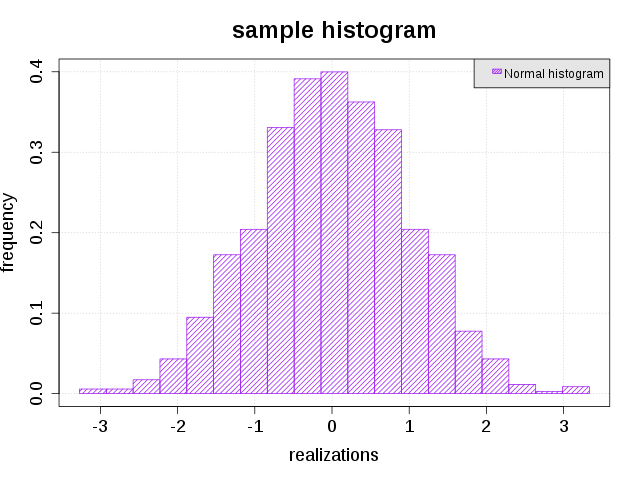
\includegraphics[width=7cm]{Figures/hist_Data.png}
                   \caption{Histogram from a sample.}
                   \label{HistogramData}
                 \end{center}
               \end{minipage}
               \hfill
               \begin{minipage}{9.8cm}
                 \begin{center}
                   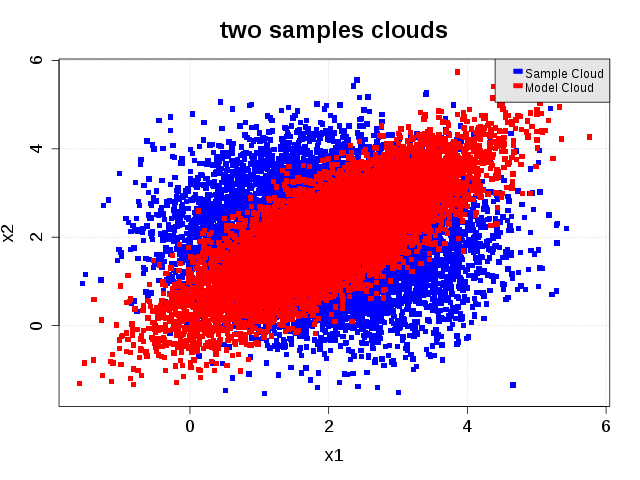
\includegraphics[width=7cm]{Figures/cloud1.png}
                   \caption{Superposition of two 2D clouds.}
                   \label{superpositionTwoclouds}
                 \end{center}
               \end{minipage}
             \end{figure}
